% Created by tikzDevice version 0.12.6 on 2024-05-22 16:04:41
% !TEX encoding = UTF-8 Unicode
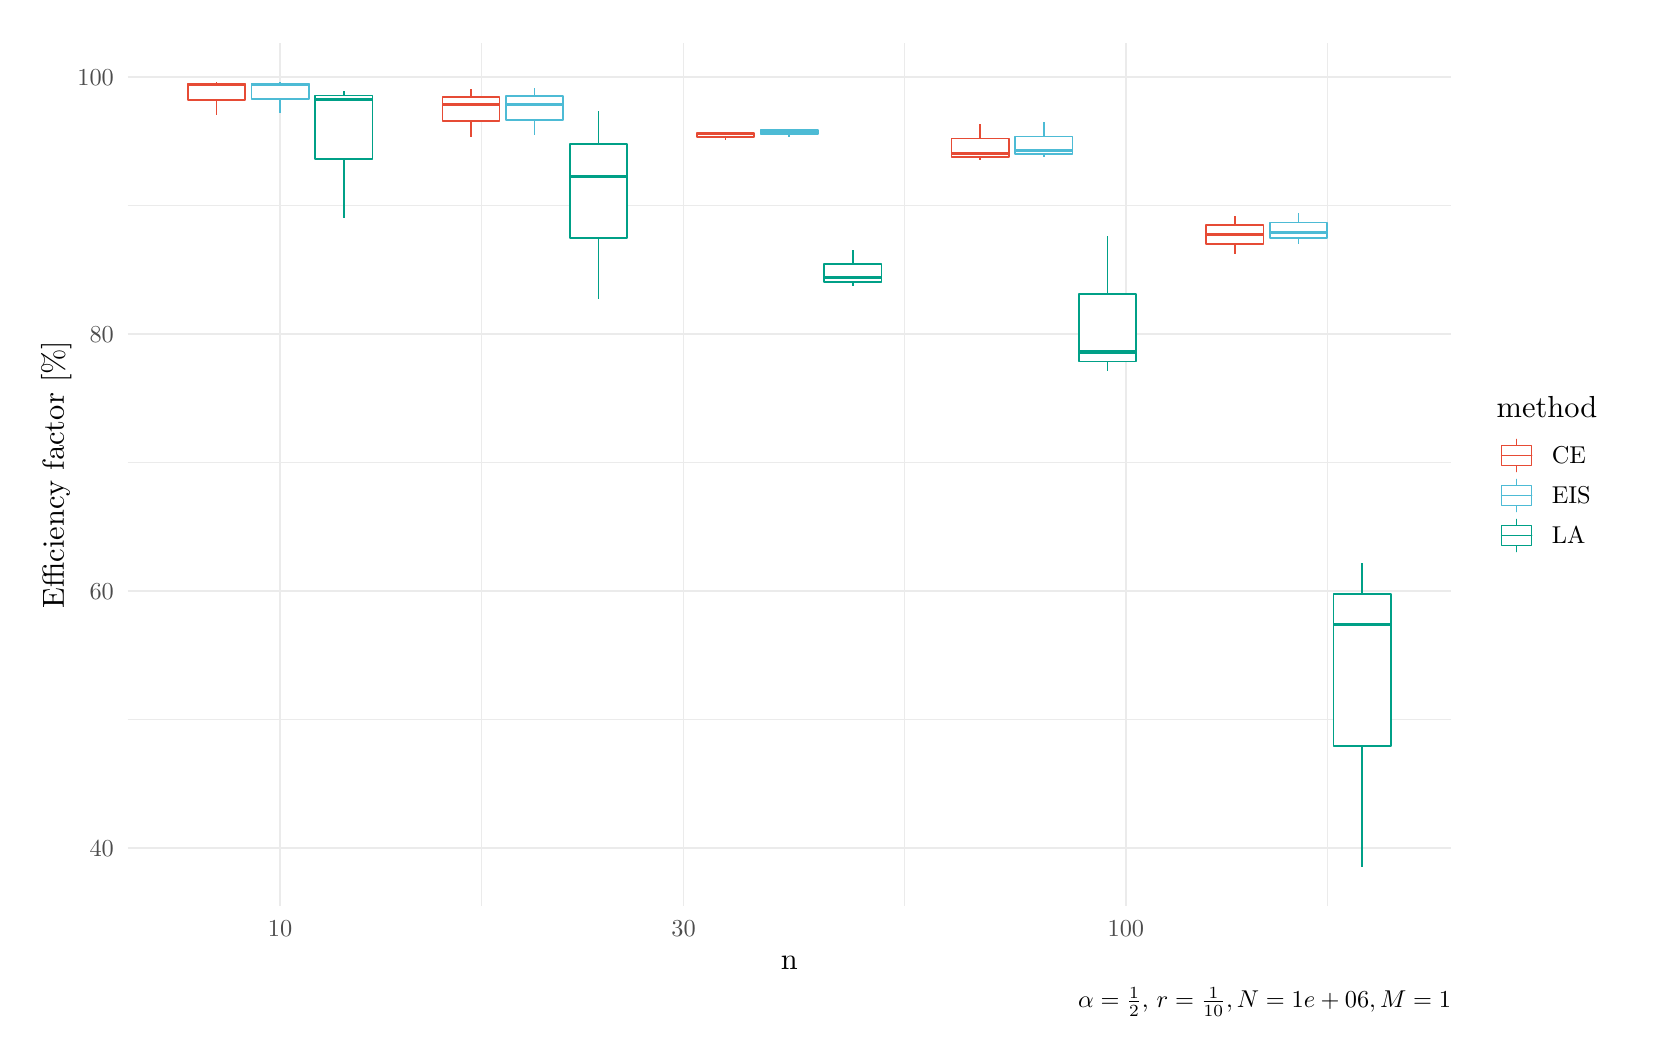
\begin{tikzpicture}[x=1pt,y=1pt]
\definecolor{fillColor}{RGB}{255,255,255}
\path[use as bounding box,fill=fillColor,fill opacity=0.00] (0,0) rectangle (578.16,361.35);
\begin{scope}
\path[clip] ( 36.11, 43.96) rectangle (514.31,355.85);
\definecolor{drawColor}{gray}{0.92}

\path[draw=drawColor,line width= 0.3pt,line join=round] ( 36.11,111.44) --
	(514.31,111.44);

\path[draw=drawColor,line width= 0.3pt,line join=round] ( 36.11,204.24) --
	(514.31,204.24);

\path[draw=drawColor,line width= 0.3pt,line join=round] ( 36.11,297.03) --
	(514.31,297.03);

\path[draw=drawColor,line width= 0.3pt,line join=round] (164.11, 43.96) --
	(164.11,355.85);

\path[draw=drawColor,line width= 0.3pt,line join=round] (316.93, 43.96) --
	(316.93,355.85);

\path[draw=drawColor,line width= 0.3pt,line join=round] (469.75, 43.96) --
	(469.75,355.85);

\path[draw=drawColor,line width= 0.6pt,line join=round] ( 36.11, 65.04) --
	(514.31, 65.04);

\path[draw=drawColor,line width= 0.6pt,line join=round] ( 36.11,157.84) --
	(514.31,157.84);

\path[draw=drawColor,line width= 0.6pt,line join=round] ( 36.11,250.63) --
	(514.31,250.63);

\path[draw=drawColor,line width= 0.6pt,line join=round] ( 36.11,343.43) --
	(514.31,343.43);

\path[draw=drawColor,line width= 0.6pt,line join=round] ( 91.20, 43.96) --
	( 91.20,355.85);

\path[draw=drawColor,line width= 0.6pt,line join=round] (237.02, 43.96) --
	(237.02,355.85);

\path[draw=drawColor,line width= 0.6pt,line join=round] (396.83, 43.96) --
	(396.83,355.85);
\definecolor{drawColor}{RGB}{230,75,53}

\path[draw=drawColor,line width= 0.6pt,line join=round] ( 68.20,341.16) -- ( 68.20,341.61);

\path[draw=drawColor,line width= 0.6pt,line join=round] ( 68.20,335.16) -- ( 68.20,329.63);
\definecolor{fillColor}{RGB}{255,255,255}

\path[draw=drawColor,line width= 0.6pt,line join=round,line cap=round,fill=fillColor] ( 57.85,341.16) --
	( 57.85,335.16) --
	( 78.55,335.16) --
	( 78.55,341.16) --
	( 57.85,341.16) --
	cycle;

\path[draw=drawColor,line width= 1.1pt,line join=round] ( 57.85,340.70) -- ( 78.55,340.70);

\path[draw=drawColor,line width= 0.6pt,line join=round] (160.20,336.32) -- (160.20,339.21);

\path[draw=drawColor,line width= 0.6pt,line join=round] (160.20,327.67) -- (160.20,321.93);

\path[draw=drawColor,line width= 0.6pt,line join=round,line cap=round,fill=fillColor] (149.85,336.32) --
	(149.85,327.67) --
	(170.55,327.67) --
	(170.55,336.32) --
	(149.85,336.32) --
	cycle;

\path[draw=drawColor,line width= 1.1pt,line join=round] (149.85,333.42) -- (170.55,333.42);

\path[draw=drawColor,line width= 0.6pt,line join=round] (252.21,323.35) -- (252.21,323.55);

\path[draw=drawColor,line width= 0.6pt,line join=round] (252.21,321.91) -- (252.21,320.66);

\path[draw=drawColor,line width= 0.6pt,line join=round,line cap=round,fill=fillColor] (241.86,323.35) --
	(241.86,321.91) --
	(262.56,321.91) --
	(262.56,323.35) --
	(241.86,323.35) --
	cycle;

\path[draw=drawColor,line width= 1.1pt,line join=round] (241.86,323.15) -- (262.56,323.15);

\path[draw=drawColor,line width= 0.6pt,line join=round] (344.21,321.24) -- (344.21,326.66);

\path[draw=drawColor,line width= 0.6pt,line join=round] (344.21,314.60) -- (344.21,313.39);

\path[draw=drawColor,line width= 0.6pt,line join=round,line cap=round,fill=fillColor] (333.86,321.24) --
	(333.86,314.60) --
	(354.56,314.60) --
	(354.56,321.24) --
	(333.86,321.24) --
	cycle;

\path[draw=drawColor,line width= 1.1pt,line join=round] (333.86,315.82) -- (354.56,315.82);

\path[draw=drawColor,line width= 0.6pt,line join=round] (436.22,289.95) -- (436.22,293.12);

\path[draw=drawColor,line width= 0.6pt,line join=round] (436.22,283.19) -- (436.22,279.59);

\path[draw=drawColor,line width= 0.6pt,line join=round,line cap=round,fill=fillColor] (425.87,289.95) --
	(425.87,283.19) --
	(446.57,283.19) --
	(446.57,289.95) --
	(425.87,289.95) --
	cycle;

\path[draw=drawColor,line width= 1.1pt,line join=round] (425.87,286.78) -- (446.57,286.78);
\definecolor{drawColor}{RGB}{77,187,213}

\path[draw=drawColor,line width= 0.6pt,line join=round] ( 91.20,341.20) -- ( 91.20,341.67);

\path[draw=drawColor,line width= 0.6pt,line join=round] ( 91.20,335.54) -- ( 91.20,330.36);

\path[draw=drawColor,line width= 0.6pt,line join=round,line cap=round,fill=fillColor] ( 80.85,341.20) --
	( 80.85,335.54) --
	(101.55,335.54) --
	(101.55,341.20) --
	( 80.85,341.20) --
	cycle;

\path[draw=drawColor,line width= 1.1pt,line join=round] ( 80.85,340.72) -- (101.55,340.72);

\path[draw=drawColor,line width= 0.6pt,line join=round] (183.20,336.54) -- (183.20,339.45);

\path[draw=drawColor,line width= 0.6pt,line join=round] (183.20,328.06) -- (183.20,322.49);

\path[draw=drawColor,line width= 0.6pt,line join=round,line cap=round,fill=fillColor] (172.85,336.54) --
	(172.85,328.06) --
	(193.55,328.06) --
	(193.55,336.54) --
	(172.85,336.54) --
	cycle;

\path[draw=drawColor,line width= 1.1pt,line join=round] (172.85,333.63) -- (193.55,333.63);

\path[draw=drawColor,line width= 0.6pt,line join=round] (275.21,324.28) -- (275.21,324.68);

\path[draw=drawColor,line width= 0.6pt,line join=round] (275.21,322.93) -- (275.21,321.97);

\path[draw=drawColor,line width= 0.6pt,line join=round,line cap=round,fill=fillColor] (264.86,324.28) --
	(264.86,322.93) --
	(285.56,322.93) --
	(285.56,324.28) --
	(264.86,324.28) --
	cycle;

\path[draw=drawColor,line width= 1.1pt,line join=round] (264.86,323.89) -- (285.56,323.89);

\path[draw=drawColor,line width= 0.6pt,line join=round] (367.21,321.97) -- (367.21,327.12);

\path[draw=drawColor,line width= 0.6pt,line join=round] (367.21,315.76) -- (367.21,314.70);

\path[draw=drawColor,line width= 0.6pt,line join=round,line cap=round,fill=fillColor] (356.86,321.97) --
	(356.86,315.76) --
	(377.57,315.76) --
	(377.57,321.97) --
	(356.86,321.97) --
	cycle;

\path[draw=drawColor,line width= 1.1pt,line join=round] (356.86,316.83) -- (377.57,316.83);

\path[draw=drawColor,line width= 0.6pt,line join=round] (459.22,290.94) -- (459.22,294.43);

\path[draw=drawColor,line width= 0.6pt,line join=round] (459.22,285.40) -- (459.22,283.34);

\path[draw=drawColor,line width= 0.6pt,line join=round,line cap=round,fill=fillColor] (448.87,290.94) --
	(448.87,285.40) --
	(469.57,285.40) --
	(469.57,290.94) --
	(448.87,290.94) --
	cycle;

\path[draw=drawColor,line width= 1.1pt,line join=round] (448.87,287.45) -- (469.57,287.45);
\definecolor{drawColor}{RGB}{0,160,135}

\path[draw=drawColor,line width= 0.6pt,line join=round] (114.20,336.83) -- (114.20,338.40);

\path[draw=drawColor,line width= 0.6pt,line join=round] (114.20,313.98) -- (114.20,292.70);

\path[draw=drawColor,line width= 0.6pt,line join=round,line cap=round,fill=fillColor] (103.85,336.83) --
	(103.85,313.98) --
	(124.55,313.98) --
	(124.55,336.83) --
	(103.85,336.83) --
	cycle;

\path[draw=drawColor,line width= 1.1pt,line join=round] (103.85,335.27) -- (124.55,335.27);

\path[draw=drawColor,line width= 0.6pt,line join=round] (206.21,319.38) -- (206.21,331.36);

\path[draw=drawColor,line width= 0.6pt,line join=round] (206.21,285.40) -- (206.21,263.40);

\path[draw=drawColor,line width= 0.6pt,line join=round,line cap=round,fill=fillColor] (195.85,319.38) --
	(195.85,285.40) --
	(216.56,285.40) --
	(216.56,319.38) --
	(195.85,319.38) --
	cycle;

\path[draw=drawColor,line width= 1.1pt,line join=round] (195.85,307.41) -- (216.56,307.41);

\path[draw=drawColor,line width= 0.6pt,line join=round] (298.21,275.93) -- (298.21,280.93);

\path[draw=drawColor,line width= 0.6pt,line join=round] (298.21,269.44) -- (298.21,267.95);

\path[draw=drawColor,line width= 0.6pt,line join=round,line cap=round,fill=fillColor] (287.86,275.93) --
	(287.86,269.44) --
	(308.56,269.44) --
	(308.56,275.93) --
	(287.86,275.93) --
	cycle;

\path[draw=drawColor,line width= 1.1pt,line join=round] (287.86,270.92) -- (308.56,270.92);

\path[draw=drawColor,line width= 0.6pt,line join=round] (390.22,265.07) -- (390.22,285.99);

\path[draw=drawColor,line width= 0.6pt,line join=round] (390.22,240.76) -- (390.22,237.38);

\path[draw=drawColor,line width= 0.6pt,line join=round,line cap=round,fill=fillColor] (379.87,265.07) --
	(379.87,240.76) --
	(400.57,240.76) --
	(400.57,265.07) --
	(379.87,265.07) --
	cycle;

\path[draw=drawColor,line width= 1.1pt,line join=round] (379.87,244.15) -- (400.57,244.15);

\path[draw=drawColor,line width= 0.6pt,line join=round] (482.22,156.79) -- (482.22,168.06);

\path[draw=drawColor,line width= 0.6pt,line join=round] (482.22,101.83) -- (482.22, 58.13);

\path[draw=drawColor,line width= 0.6pt,line join=round,line cap=round,fill=fillColor] (471.87,156.79) --
	(471.87,101.83) --
	(492.57,101.83) --
	(492.57,156.79) --
	(471.87,156.79) --
	cycle;

\path[draw=drawColor,line width= 1.1pt,line join=round] (471.87,145.53) -- (492.57,145.53);
\end{scope}
\begin{scope}
\path[clip] (  0.00,  0.00) rectangle (578.16,361.35);
\definecolor{drawColor}{gray}{0.30}

\node[text=drawColor,anchor=base east,inner sep=0pt, outer sep=0pt, scale=  0.88] at ( 31.16, 62.01) {40};

\node[text=drawColor,anchor=base east,inner sep=0pt, outer sep=0pt, scale=  0.88] at ( 31.16,154.81) {60};

\node[text=drawColor,anchor=base east,inner sep=0pt, outer sep=0pt, scale=  0.88] at ( 31.16,247.60) {80};

\node[text=drawColor,anchor=base east,inner sep=0pt, outer sep=0pt, scale=  0.88] at ( 31.16,340.40) {100};
\end{scope}
\begin{scope}
\path[clip] (  0.00,  0.00) rectangle (578.16,361.35);
\definecolor{drawColor}{gray}{0.30}

\node[text=drawColor,anchor=base,inner sep=0pt, outer sep=0pt, scale=  0.88] at ( 91.20, 32.95) {10};

\node[text=drawColor,anchor=base,inner sep=0pt, outer sep=0pt, scale=  0.88] at (237.02, 32.95) {30};

\node[text=drawColor,anchor=base,inner sep=0pt, outer sep=0pt, scale=  0.88] at (396.83, 32.95) {100};
\end{scope}
\begin{scope}
\path[clip] (  0.00,  0.00) rectangle (578.16,361.35);
\definecolor{drawColor}{RGB}{0,0,0}

\node[text=drawColor,anchor=base,inner sep=0pt, outer sep=0pt, scale=  1.10] at (275.21, 20.91) {n};
\end{scope}
\begin{scope}
\path[clip] (  0.00,  0.00) rectangle (578.16,361.35);
\definecolor{drawColor}{RGB}{0,0,0}

\node[text=drawColor,rotate= 90.00,anchor=base,inner sep=0pt, outer sep=0pt, scale=  1.10] at ( 13.08,199.90) {Efficiency factor [\%]};
\end{scope}
\begin{scope}
\path[clip] (  0.00,  0.00) rectangle (578.16,361.35);
\definecolor{drawColor}{RGB}{0,0,0}

\node[text=drawColor,anchor=base west,inner sep=0pt, outer sep=0pt, scale=  1.10] at (530.81,220.55) {method};
\end{scope}
\begin{scope}
\path[clip] (  0.00,  0.00) rectangle (578.16,361.35);
\definecolor{drawColor}{RGB}{230,75,53}

\path[draw=drawColor,line width= 0.6pt,line join=round,line cap=round] (538.03,200.97) --
	(538.03,203.14);

\path[draw=drawColor,line width= 0.6pt,line join=round,line cap=round] (538.03,210.36) --
	(538.03,212.53);
\definecolor{fillColor}{RGB}{255,255,255}

\path[draw=drawColor,line width= 0.6pt,line join=round,line cap=round,fill=fillColor] (532.61,203.14) rectangle (543.45,210.36);

\path[draw=drawColor,line width= 0.6pt,line join=round,line cap=round] (532.61,206.75) --
	(543.45,206.75);
\end{scope}
\begin{scope}
\path[clip] (  0.00,  0.00) rectangle (578.16,361.35);
\definecolor{drawColor}{RGB}{77,187,213}

\path[draw=drawColor,line width= 0.6pt,line join=round,line cap=round] (538.03,186.51) --
	(538.03,188.68);

\path[draw=drawColor,line width= 0.6pt,line join=round,line cap=round] (538.03,195.91) --
	(538.03,198.08);
\definecolor{fillColor}{RGB}{255,255,255}

\path[draw=drawColor,line width= 0.6pt,line join=round,line cap=round,fill=fillColor] (532.61,188.68) rectangle (543.45,195.91);

\path[draw=drawColor,line width= 0.6pt,line join=round,line cap=round] (532.61,192.30) --
	(543.45,192.30);
\end{scope}
\begin{scope}
\path[clip] (  0.00,  0.00) rectangle (578.16,361.35);
\definecolor{drawColor}{RGB}{0,160,135}

\path[draw=drawColor,line width= 0.6pt,line join=round,line cap=round] (538.03,172.06) --
	(538.03,174.23);

\path[draw=drawColor,line width= 0.6pt,line join=round,line cap=round] (538.03,181.46) --
	(538.03,183.62);
\definecolor{fillColor}{RGB}{255,255,255}

\path[draw=drawColor,line width= 0.6pt,line join=round,line cap=round,fill=fillColor] (532.61,174.23) rectangle (543.45,181.46);

\path[draw=drawColor,line width= 0.6pt,line join=round,line cap=round] (532.61,177.84) --
	(543.45,177.84);
\end{scope}
\begin{scope}
\path[clip] (  0.00,  0.00) rectangle (578.16,361.35);
\definecolor{drawColor}{RGB}{0,0,0}

\node[text=drawColor,anchor=base west,inner sep=0pt, outer sep=0pt, scale=  0.88] at (550.76,203.72) {CE};
\end{scope}
\begin{scope}
\path[clip] (  0.00,  0.00) rectangle (578.16,361.35);
\definecolor{drawColor}{RGB}{0,0,0}

\node[text=drawColor,anchor=base west,inner sep=0pt, outer sep=0pt, scale=  0.88] at (550.76,189.27) {EIS};
\end{scope}
\begin{scope}
\path[clip] (  0.00,  0.00) rectangle (578.16,361.35);
\definecolor{drawColor}{RGB}{0,0,0}

\node[text=drawColor,anchor=base west,inner sep=0pt, outer sep=0pt, scale=  0.88] at (550.76,174.81) {LA};
\end{scope}
\begin{scope}
\path[clip] (  0.00,  0.00) rectangle (578.16,361.35);
\definecolor{drawColor}{RGB}{0,0,0}

\node[text=drawColor,anchor=base east,inner sep=0pt, outer sep=0pt, scale=  0.88] at (514.31,  7.21) {$\alpha = \frac 1 2$, $r = \frac 1 {10}, N = 1e+06, M=1$};
\end{scope}
\end{tikzpicture}
